\chapter{Quantifying sensitivities of satellite-simulated cloud retrievals to unresolved clouds and precipitation}\label{sg_chapter}

The simulator framework is essentially a means for accounting for uncertainties, biases, and limitations in satellite retrievals of cloud properties in order to make more consistent comparisons with modeled cloud properties. However, because the descriptions of clouds in GCMs are themselves limited and insufficient for directly simulating the satellite retrievals, the process of simulating satellite retrieval products relies on additional assumptions about the model clouds beyond the descriptions provided by the models themselves. This introduces another layer of complexity and another possible source for errors or ambiguities.

At the heart of this problem is the fact that while cloud properties in the physical atmosphere vary at all spatial scales down to (and below) those measured by satellite sensors, the current resolution of most global climate models is limited by computational expense and model infrastructure to hundreds of kilometers. For example, climate model simulations produced for the latest round of the Climate Model Intercomparison Project (CMIP5; [citations]) and referenced in the Intergovernmental Panel on Climate Change (IPCC) AR5 used grids with typical resolutions of 1 to 2 degrees \citep{flato_et_al_2013}, which translates to about 100-200 km at the equator. Because of these coarse-scale grids, current large-scale models cannot explicitly resolve individual cloud elements at the scales observed by satellites (1-2 km for the MISR and CloudSat retrievals used predominantly in this study), but rather must rely on (often empirically-based) statistical parameterizations about the nature of clouds at these larger scales that summarize the aggregated properties of the smaller scales \citep{randall_et_al_2003}.

As stated by \cite{pincus_et_al_2012} and mentioned in Chapter \ref{introduction_chapter}, the relatively coarse resolution of GCMs is problematic because the gridbox-mean description of clouds implies a distribution of possible simulated retrievals within each gridbox. The gridbox mean description of clouds does not in itself specify how the clouds should be distributed horizontally and vertically within model gridboxes, and thus characterization of the unresolved structure depends on additional assumptions about how clouds in overlapping layers are aligned vertically and how cloud properties vary within model gridboxes.

The importance of unresolved cloud properties is not unique to the problem of simulating satellite retrievals, but is more generally important to the problem of calculating radiative fluxes and heating rates within models. This is due to the fact that radiative fluxes are non-local. That is, the radiative flux resulting from a combination of two layers depends on the degree to which those two layers overlap vertically. %Because the incremental increase in albedo is smaller for larger optical depths, the combined albedo for two overlapping layers is smaller than that for two non-overlapping layers. Likewise, outgoing longwave fluxes are non-linea
Many early radiative transfer parameterizations in large-scale models accounted for the overlapping nature of clouds from partly cloudy layers by appropriately weighting clear and cloudy-sky flux calculations to satisfy a specific overlap assumption. These overlap assumptions were necessarily simply defined, and have included random overlap, in which clouds in different vertical layers are assumed to be completely uncorrelated, maximum overlap, in which clouds in different layers are assumed to be perfectly correlated (or ``lined up''), and the popular maximum-random overlap, in which clouds in adjacent cloudy (or continuous) layers are maximimally overlapped and clouds in layers separated by at least one clear layer are randomly overlapped \citep{geleyn_and_hollingsworth_1979, tian_and_curry_1989}. The maximum-random overlap in particular has been used in a number of GCMs \citep[e.g.,][]{collins_et_al_2004, neale_et_al_2010a, neale_et_al_2010b}. That different overlap assumptions can significantly affect simulated radiative quantities is well established \citep[e.g.,][]{morcrette_and_fouquart_1986, stubenrauch_et_al_1997, barker_et_al_1999}, and these overly simple assumptions have been shown insufficient in capturing the complexity of cloud overlap seen in observations \citep{hogan_and_illingworth_2000, mace_and_benson-troth_2002, barker_2008} and in high-resolution model simulations [citations]. Sensitivity tests using high resolution model simulations have shown that these unrealistic overlap assumptions can lead to instantaneous errors in calculated fluxes in excess of 50 W/m$^2$ \citep{barker_et_al_1999, wu_and_liang_2005}, suggesting that a more realistic treatment of cloud overlap should be sought for inclusion in GCMs. %\cite{oreopoulos_et_al_2012} demonstrate more modest (but still important) global mean errors on the order of 4 W/m$^2$ in cloud radiative effects in a GCM.

Subgrid-scale horizontal variability in cloud condensate is often completely neglected (or poorly represented by simple scaling of optical depths, e.g. [citations]) in GCMs, despite the fact that clouds can exhibit large horizontal variability on scales much smaller than GCM gridboxes \citep[e.g.,][]{stephens_and_platt_1987}. This is problematic because radiative fluxes and heating rates calculated from model radiative transfer parameterizations are sensitive to subgrid-scale variations in cloud condensate \citep[e.g.,][]{barker_et_al_1999,wu_and_liang_2005,oreopoulos_et_al_2012}. \cite{barker_et_al_1999} demonstrate instantaneous flux errors due to unresolved horizontal cloud variability in excess of $100 ~\text{W}/\text{m}^2$, and \cite{oreopoulos_et_al_2012} demonstrate global cloud radiative effect errors on the order of $5 ~\text{W}/\text{m}^2$, with much larger regional errors. The sensitivity to both cloud overlap and condensate horizontal variability emphasizes the need to provide descriptions of clouds in large-scale model radiative calculations that include both horizontal variability in cloud properties and more realistic cloud overlap.

An alternative to the approach of weighting clear and cloudy sky fluxes is to generate stochastic samples of binary clear or cloudy ``subcolumn'' profiles such that in the limit of many such samples the gridbox-mean partial cloudiness profile is reproduced and the subcolumn profiles are consistent with an assumed overlap. This approach, described by \cite{klein_and_jakob_1999} to generate stochastic subcolumns for use with the ISCCP simulator, provides psuedo-resolved cloud fields sufficient for not only simulating satellite retrievals, but also for performing radiative transfer calculations using the independent column approximation \citep[ICA;][]{cahalan_et_al_1994}. \cite{barker_et_al_2002} and \cite{pincus_et_al_2003} made this approach for calculating fluxes and heating rates much more tractable for use in large-scale models by introducing the Monte Carlo Independent Column Approximation (McICA), in which both cloud state (subcolumns) and spectral interval are stochastically sampled simultaneously, drastically reducing the computational burden associated with integrating calculations over a large number of spectral intervals for each column. This allows for fast ICA-like radiative transfer calculations (at the expense of artificially increased random noise) and more flexible representations of subgrid-scale cloud structure, and has since been incorporated into the widely used RRTMG radiation package and used in a number of state-of-the-art models \citep{iacono_et_al_2008, von_salzen_et_al_2012, neale_et_al_2010a, neale_et_al_2010b, donner_et_al_2011, hogan_et_al_2014}.

McICA separates the treatment of cloud structure and variability from radiative transfer parameterization, leaving the task of describing complex cloud structure and variability up to subcolumn sampling schemes. In principle, arbitrarily complex cloud geometries and condensate distributions can be generated by incorporating more sophisticated subcolumn schemes. However, the subcolumn schemes currently used in most GCMs make many of the same simplifications used by earlier models, including maximum-random overlap and homogeneous cloud properties \citep[e.g.,][]{neale_et_al_2010a, neale_et_al_2010b}. Improved subcolumn schemes are needed to take full advantage of the flexibility offered by McICA.

%Unresolved cloud structure and condensate variability is important not only for calculations of radiative fluxes, but also for cloud diagnostics commonly used for evaluation of model cloud properties themselves. Satellite instrument simulators such as those provided by the CFMIP Observational Simulator Package \citep[COSP;][]{bodas-salcedo_et_al_2011} are often used to remove ambiguities in model evaluation studies that arise from uncertainties and limitations in satellite retrievals of cloud properties by producing psuedo-observations from the model state that are more directly comparable to the satellite observations \citep[e.g.,][]{klein_and_jakob_1999,webb_et_al_2001,zhang_et_al_2005,zhang_et_al_2010,kay_et_al_2012,klein_et_al_2013}. A key first step in simulating satellite observations from GCM cloud properties is accounting for the mismatch in resolved scales between the satellite pixel and model resolution by downscaling the gridbox mean cloud properties. This is done in COSP by stochastically generating subcolumns consistent with an overlap assumption to account for correlations in overlapping cloudy layers in the same manner as described for McICA above. However, the current implementation of COSP allows for only the simple maximum, random, or maximum-random overlap, and treats subcolumn clouds and precipitation as homogeneous. Furthermore, while the subcolumn treatent in COSP is intended to account for the mismatch in resolved scales between satellite pixel and model resolutions, a specific spatial scale in terms of the number of subcolumns chosen is not defined within the COSP subcolumn treatment. Condensate variability will need to be tied to an explicit scale. Also, previous studies have shown that overlap statistics are dependent on resolution \citep[e.g.,][]{mace_and_benson-troth_2002}, and so the number of subcolumns chosen within COSP should be defined in terms of model resolution in order to correctly match scales.

As discussed in Chapter \ref{introduction_chapter}, the first step in simulating satellite retrievals from GCM output is to downscale the gridbox-mean quanitities to scales approximating those at which the actual satellite retrievals are performed. In COSP, this is done by generating stochastic subcolumns following \cite{klein_and_jakob_1999}, analogous to how subcolumns are generated for McICA, following the simple overlap assumptions described above with horizontally homogeneous cloud condensate. To the extent that the simulated satellite retrievals are sensitive to these assumptions, failing to accurately characterize the subgrid cloud structure and condensate variability potentially introduces ambiguities into satellite-model comparisons. The sensitivity of the satellite-simulated cloud properties to assumptions about unresolved cloud and precipitation are quantified here, and a framework for reducing errors due to these assumptions is presented in Chapter \ref{sgi_chapter}.

%show in this chapter that these assumptions also lead to intrinsic errors in simulated satellite cloud diagnostics. I use high-resolution model output from the Multi-scale Modeling Framework \citep[MMF;][]{randall_et_al_2003}, which embeds a 2D cloud resolving model (CRM) into each gridbox of a traditional GCM, to provide baseline cloud-resolved fields with global coverage. I then create a series of modified cases from the CRM fields to mimic the assumptions of homogeneous cloud and precipitation properties and the maximum-random overlap assumption ubiquitous in current global climate model radiative codes. Both the modified and unmodified CRM fields are run through the Cloud Feedback Model Intercomparison Project (CFMIP) Observational Simulator Package (COSP; Bodas-Salcedo et al. 2011) to calculate simulated satellite cloud diagnostics, and diagnostics from the modified and unmodified fields are compared to evaluate the sensitivity to the homogeneous and overlap assumptions. [need to significantly clean up this paragraph and the remainder of the introduction]

%Cloud cover, the fraction of surface area covered by one or more cloud layers, is often used as a measure of the amount of cloud present. However, even this seemingly simple quantity is dependent upon the scale at which it is measured or defined \citep{digirolamo_and_davies_1997, zhao_and_digirolamo_2006}. Satellite imagers often retrieve an albedo or optical depth-like quantity that quantifies cloud solar reflectance that, taken together with cloud cover, can be useful in understanding the radiative impact of clouds. In fact simultaneous evaluation of cloud cover and optical depth in models has led to the diagnosis of a prevalent tendency for models to overestimate cloud optical depth while underestimating cloud cover \citep{webb_et_al_2001, weare_2004, zhang_et_al_2005, nam_et_al_2012, kay_et_al_2012, klein_et_al_2013}. But satellite-retrieved optical depth is also dependent on scale, and in particular is dependent on the horizontal extent of clouds \citep[e.g.,][]{evans_et_al_2008}.

\section{Framework for sensitivity tests}\label{section_sg_framework}
Simulating satellite cloud diagnostics from coarse-resolution large-scale model output using COSP is a multi-step process. First, profiles of partial cloudiness (cloud fraction) from each gridbox of the model are represented by an array of columns (typically called subcolumns), where individual elements in the array are considered either fully clear or fully cloudy (that is, cloud fraction is equal to zero or one at each level in each subcolumn). The cloud elements are arranged (or ``overlapped'') consistent with a given overlap assumption (intended to be consistent with that used in the model radiative scheme, often maximum-random). This ``subcolumn generation'' is handled by the COSP Subgrid Cloud Overlap Profile Sampler \citep[SCOPS;][]{klein_and_jakob_1999} routine. In current versions of COSP, the condensate and cloud optical properties of each cloudy element are fixed to the model gridbox mean (within each vertical layer). Subcolumn precipitation occurrence is diagnosed from the subcolumn cloud occurrence and either the precipitation condensate amount or the precipitation flux using the set of rules described by \cite{zhang_et_al_2010} and implemented in the {\tt PREC\_SCOPS} routine. In that routine, subcolumn precipitation is assumed to maximally overlap with cloud where gridbox precipitation condensate or fluxes are non-zero, and precipitation condensate is fixed to the model gridbox mean within each vertical layer. The individual satellite simulator algorithms are then performed on these profiles, producing a set of pseudo-retrievals at the subcolumn scale. Lastly, these pseudo-retrievals are aggregated into statistical summaries that can be directly compared with available observational products from specific satellites.

The generation of subcolumn cloud and precipitation profiles described above is consistent with the approach used in radiative schemes in current GCMs that use the Monte Carlo Independent Column Approximation \citep[McICA;][]{pincus_et_al_2003}. This approach typically makes two fundamental assumptions about the unresolved cloud and precipitation properties: that cloud and precipitation occurrence overlap can be treated using simple overlap rules, and that cloud and precipitation condensate can be treated as homogeneous at the gridbox scale, such that subcolumn condensate amounts can be fixed by the gridbox mean values at each vertical level. The homogeneous condensate assumption, however, has been shown to lead to errors in calculated domain-average fluxes and heating rates \citep[e.g.,][]{barker_et_al_1999}, and other investigators have started to explore more realistic treatments of small-scale cloud properties in large-scale models \citep[e.g.,][]{oreopoulos_et_al_2012, von_salzen_et_al_2012}. [much of this is redundant with the introduction; remove and/or condense this] The simple cloud overlap assumptions used in the majority of GCMs have also been recently called into question. Cloud overlap is often prescribed as one of maximum (cloudy portions of layers are perfectly correlated), random (cloudy portions of layers are uncorrelated), or the popular maximum-random overlap (hereafter referred to as ``MRO''), in which contiguous layers are maximally overlapped and non-contiguous layers (those separated by at least one completely clear layer) are randomly overlapped \citep[e.g.,][]{geleyn_and_hollingsworth_1979}. Recent studies using both ground-based \citep{mace_and_benson-troth_2002, hogan_and_illingworth_2000} and satellite-based \citep{barker_2008} cloud radar and lidar have shown, however, that MRO fails to accurately capture the overlap statistics of observed clouds.  In particular, these studies have shown that contiguous cloudy layers are somewhat less than maximally overlapped, and have suggested instead an overlap that is a linear combination of maximum and random overlap (referred to as ``generalized overlap'').

The simulation process described above assumes that grid-mean profiles of cloudiness and condensate are provided as inputs, however the modular structure of COSP enables bypassing the subcolumn generation step if resolved condensate fields with sufficiently high resolution (that approximating the scales at which the actual retrievals are performed) are available. This is done when using COSP with a cloud-resolving model, including MMF models \citep[e.g.,][]{marchand_et_al_2009, marchand_and_ackerman_2010}. Using inputs with resolved cloud properties then enables testing arbitrary assumptions about small-scale variability and overlap simply by obtaining or creating condensate fields with differing properties, passing these directly to the individual simulator routines, and comparing the COSP-simulated outputs. A similar approach has been used by previous investigators to quantify sensitivities in radiative fluxes and heating rates using cloud-resolving models to provide the initial high resolution fields, and then modifying those fields to mimic large-scale model assumptions \citep[e.g.,][]{barker_et_al_1999}. In order to evaluate how assumptions about unresolved variability affect cloud diagnostics at both regional and global scales, a larger set of inputs is sought for this study; ideally a set of cloud and precipitation fields with global coverage.

In the Multi-scale Modeling Framework \citep[MMF;][]{randall_et_al_2003} the convection and cloud parameterizations in a traditional GCM are replaced by a cloud-resolving model running within each model grid box. This concept was first implemented into the NCAR Community Atmosphere Model (CAM) using the System for Atmospheric Modeling (SAM) as the cloud resolving model \citep[SP-CAM;][]{khairoutdinov_and_randall_2001}, but has also been implemented with a completely different GCM and CRM \citep{tao_et_al_2009} and with a variety of different cloud resolving modes and schemes for handling turbulence, clouds and aerosols \citep[e.g.,][]{cheng_and_xu_2011, cheng_and_xu_2013}. MMF models provide sufficiently high resolution (approximating satellite field of view) cloud and precipitation properties within each gridbox to run the simulators within COSP without using a subcolumn generator, and also provide the global coverage necessary to evaluate the impact of modifying the inputs on both the global and regional diagnostics typically used to evaluate the performance of clouds in global climate models [citations].  For this chapter, a single month (simulated July 2000) of 3-hourly output from the SP-CAM (version 3) is used to derive the inputs to the COSP simulators. The model was run using an east-west oriented 2-dimensional cloud-resolving model with 64 columns, a 4 km horizontal resolution with 26 vertical levels, and single moment bulk microphysics scheme.  Further details of the model configuration are given by \cite{khairoutdinov_et_al_2005} and \cite{marchand_et_al_2009}.

In order to separately evaluate the sensitivity of the COSP diagnostics to occurrence overlap and condensate heterogeneity, a series of modified cloud and precipitation fields with incremental changes are created from the original CRM fields output from SAM running within SP-CAM. These modifications are described below, and total cloud and precipitation condensate amounts for each modification are shown in Figure \ref{sg_mxratio_example} for an example grid-box (00 UTC 01 July 2000, 10 N, 180 E) along with the original, unmodified CRM fields (top row in the figure).

\begin{figure}
    \centering
    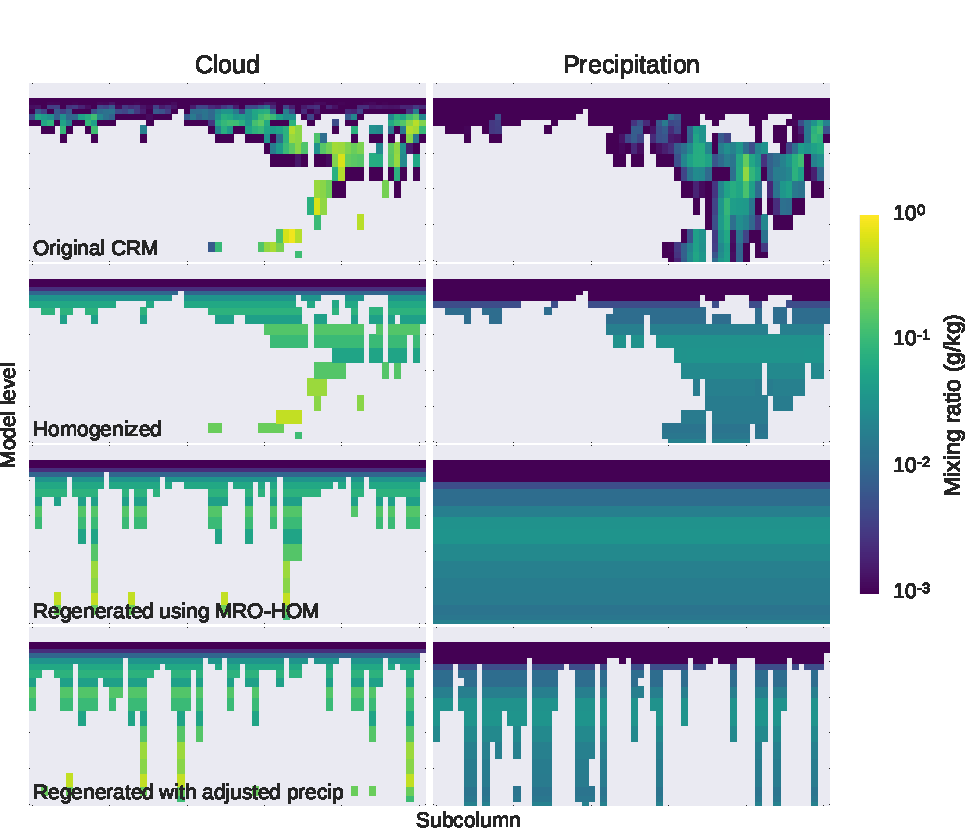
\includegraphics[width=\columnwidth]{graphics/mxratio_mro-hom.pdf}
    \caption{Total cloud (left) and precipitation (right) mixing ratios from the original CRM fields (top), homogenized CRM fields (second row), regenerated using SCOPS/PREC\_SCOPS (third row), and regenerated using SCOPS/PREC\_SCOPS with precipitation adjusted to conform to the precipitation fraction from the CRM (bottom row) for an example gridbox (00 UTC 01 July 2000, 10 N, 180 E).} 
    \label{sg_mxratio_example} 
\end{figure}

First, a set of fields with homogenized condensate (referred to as ``CRM-HOM'') is created by replacing the condensate amount in each cloudy CRM column in each gridbox with the gridbox in-cloud average (for each level). This is repeated for precipitation. No change is made to the spatial (horizontal or vertical) location of cloud and precipitation or how cloud and precipitation overlap with one another, so this modification retains the exact cloud and occurrence overlap from the original CRM.

A second set of modified fields (referred to as ``MRO-HOM'') is created by first calculating the gridbox mean cloud fraction and cloud and precipitation condensate profiles (similarly to how a GCM would represent the clouds) and then regenerating cloud and precipitation subcolumns using SCOPS and PREC\_SCOPS with maximum-random cloud overlap and homogeneous condensate.

With this set of three cases, the sensitivities of the COSP diagnostics to both occurrence overlap and condensate heterogeniety can be separately quantified by calculating appropriate differences between the three cases. Because the CRM-HOM case shares the exact occurrence overlap with the original CRM fields but uses homogenized condensate, differences in the COSP diagnostics between the CRM-HOM case and those from the unmodified CRM case will show the sensitivity of the COSP diagnostics to the assumption of homogeneous cloud and precipitation condensate. Because the MRO-HOM fields share the same homogeneous condensate profiles as the CRM-HOM fields but with maximum-random occurrence overlap, differences between MRO-HOM and CRM-HOM will show the additional impact of maximum-random occurrence overlap. Lastly, the differences between MRO-HOM and CRM will show the total error due to using both homogeneous cloud and precipitation condensate and maximum-random overlap (i.e., the GCM-equivalent errors expected using both MRO and homogeneous condensate). Symbolically, for a COSP-simulated quantity $X$ (i.e., MISR cloud top height, CloudSat reflectivity), the total error in using the subcolumn generator $E_{\rm total}$, the component of the error due to using homogeneous condensate $E_{\rm homogeneous}$, and the component of the error due to the overlap assumption $E_{\rm overlap}$ are calculated as
\begin{gather}
    E_{\rm total} = X_{\rm MRO-HOM} - X_{\rm CRM} \\
    E_{\rm homogeneous} = X_{\rm CRM-HOM} - X_{\rm CRM} \\
    E_{\rm overlap} = X_{\rm MRO-HOM} - X_{\rm CRM-HOM}
\end{gather}

While the simulators for the passive remote sensing instruments ISCCP, MODIS, and MISR take as input only the cloud properties, CloudSat radar reflectivity is extremely sensitive to the presence of precipitation (because radar reflectivity depends on the sixth moment of the particle size distribution), and thus the treatment of precipitation is critical to the accurate simulation of radar reflectivity. The public release of COSP (versions 1.4 and earlier) uses the precipitation treatment described by \cite{zhang_et_al_2010} [NOTE: some of this is redundant with the introduction to SCOPS/PREC\_SCOPS above]. The precipitation scheme (PREC\_SCOPS) takes as input the subcolumn clear/cloudy flag determined by the subcolumn cloud generator (SCOPS) and either the gridbox-mean precipitation flux or mixing ratio profiles on model levels. The algorithm steps down from the top of the atmosphere, and assigns the precipitation flag to columns based on both the cloud and precipitation flags in adjacent levels. However, there is no constraint in the algorithm on the fraction of columns that are determined to be precipitating, and Figure \ref{sg_mxratio_example} shows that this can lead to an overestimation of the number precipitating subcolumns, and it will be shown below that this leads to especially large errors in simulated CloudSat radar reflectivity and diagnostics calculated from it.

While many GCMs may not yet include precipitation fraction as model fields, it is available in the NCAR CAM model, and is easily calculated from the CRM fields in the SP-CAM model output used in this study. This enables a simple modification to the regenerated subcolumn precipitation condensate to force the fraction of precipitating subcolumns at any level within a gridbox to match the fraction of precipitating CRM columns at that level in the baseline CRM fields. This is accomplished by first using PREC\_SCOPS to generate the subcolumn precipitation flag based on the subcolumn clear/cloudy flag (from the subcolumn cloud generator, SCOPS) and the gridbox precipitation mixing ratios. Precipitation is then either systematically removed (or added, if PREC\_SCOPS underestimates the precipitation fraction) from individual subcolumns until the fraction of precipitating subcolumns matches the CRM precipitation fraction. Precipitation is preferentially removed from those subcolumns with the lowest number of cloudy levels, and is preferentially added to the subcolumns with the highest number of cloudy levels when precipitation needs to be added. This is similar to the ``PEVAP'' adjustment used by \cite{dimichele_et_al_2012}. An additional set of modified fields is created from the original CRM fields (referred to as ``MRO-HOM-PADJ'') using SCOPS with MRO, homogeneous cloud and precipitation condensate, and this precipitation adjustment. It will be shown below that this adjustment substantially reduces the errors in simulated CloudSat radar reflectivity.

In order to more easily evaluate the properties of the modified fields, and to ensure a consistent treatment for each case, the modified cases are created outside of the COSP software infrastructure, and then fed into COSP via a standalone driver program. COSP is intended to be implemented directly into the source code of a model, but a minimal working driver program capable of reading in archived large-scale model output in netCDF format and saving COSP outputs in CMOR-compliant netCDF files is distributed with the COSP source code. In order to run COSP on the SP-CAM output used in this study, this minimal example program was substantially rewritten and modularized, resulting in a stand-alone Fortran 90 program that can read standard history files from SP-CAM and write COSP outputs in CMOR-compliant format as well.

[include?]Because all of the analysis for this work was done in Python using the Scientific Python Ecosystem, an additional program was developed that bypasses the intermediate step of re-writing the modified cases to netCDF files themselves and instead calls COSP directly. This was accomplished by first adapting the example driver program provided with COSP into a callable subroutine. This subroutine was then compiled using the F2PY utility to create a shared library callable from Python. A thin wrapper was then written around the subroutine to take SP-CAM-like fields and conform them to the input format expected using transposing and reshaping operations. The wrapper then collects the COSP outputs into structures containing both the output data and metadata using the ``xarray'' [citation] Python library. This software has been published as open source, and is available for download at [...].

\section{Sensitivity of simulated passive remote sensing diagnostics} 
[much of this should have already been described in previous chapters] The MISR, ISCCP, and MODIS simulators estimate the cloud top heights (or cloud top pressures, in the case of ISCCP and MODIS) that would be retrieved by each instrument from the model input. These cloud top heights are aggregated together with the column cloud optical depth into joint histograms consistent with those produced by the individual instrument teams. These diagnostic summaries provide a description of cloud occurrence tied to their radiative impact, because the height of cloud top affects top of atmosphere outgoing longwave emission (and heating of the surface and atmosphere below the cloud top) and the optical depth or brightness of clouds affects the reflectance of shortwave energy to space (and cooling of the surface and atmosphere below cloud top). Cloud area can be calculated from these joint histograms by summing appropriate bins in the joint histograms. 

\begin{figure}
\centering
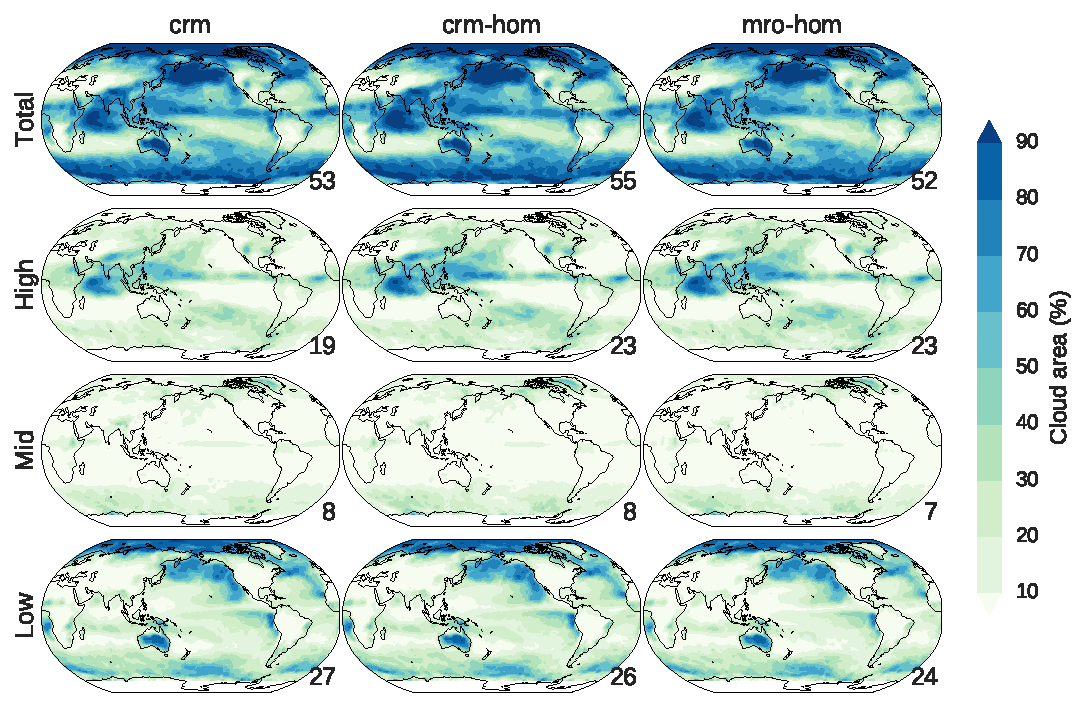
\includegraphics[width=\columnwidth]{graphics/cldmisr_mro-hom.pdf}
\caption{From top to bottom, MISR-simulated total, high-topped, mid-topped, and low-topped cloud area using the (from left to right) CRM, CRM-HOM, and MRO-HOM fields as input to COSP.}
\label{sg_cldmisr_maps}
\end{figure}

Figure \ref{sg_cldmisr_maps} shows MISR-simulated monthly-mean total (optical depth $\tau > 0.3$), high-topped (cloud top height $z_c > 7$ km, $\tau > 0.3$), mid-topped ($3 < z_c < 7$ km, $\tau > 0.3$), and low-topped ($z_c < 3$ km, $\tau > 0.3$) cloud area simulated from the baseline CRM, CRM-HOM, and MRO-HOM cases. The spatial patterns and global means are similar between each of these cases, and global mean values agree to within 4\% cloud area. While the differences in the global means appear small, it should be noted that this is on the order of the uncertainty in comparisons between MISR retrievals and MISR-simulated retrievals using CloudSat and CALIPSO-derived extinction profiles, as shown in Chapter \ref{me_chapter} and \cite{hillman_et_al_2016}. It will also be shown in Chapter \ref{cmip5_chapter} that mid and high-topped clouds in many of the CMIP5 models evaluated have global mean biases on the order of 5\% cloud area, so these errors are comparable.

\begin{figure}
\centering
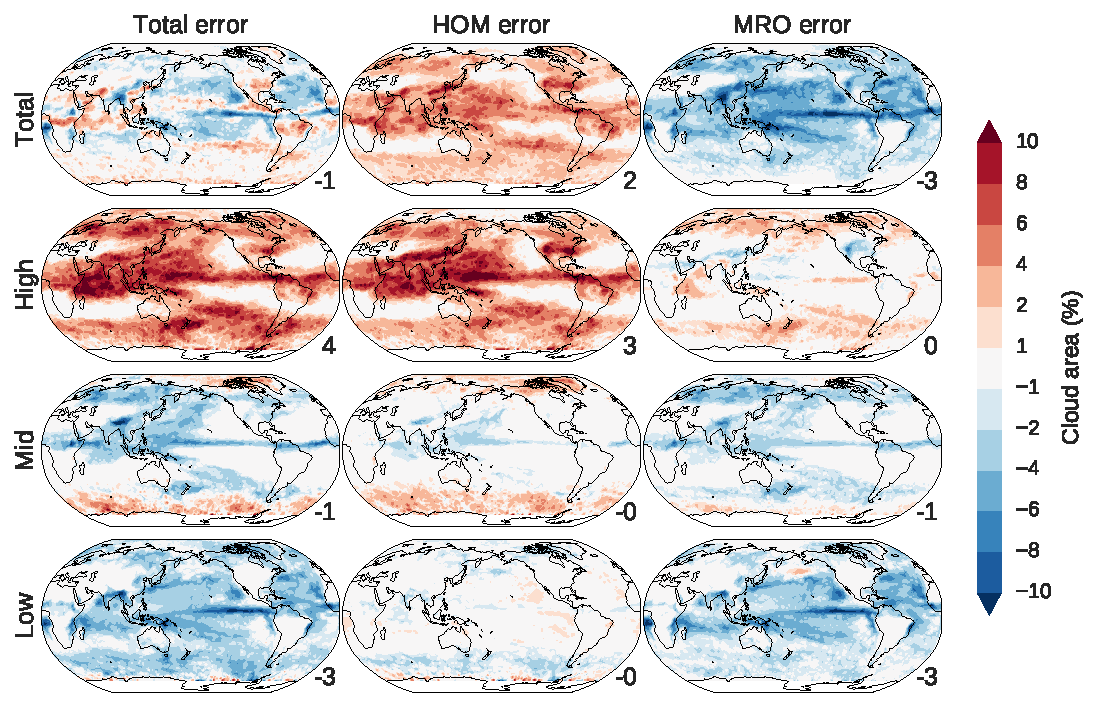
\includegraphics[width=\columnwidth]{graphics/cldmisr_mro-hom_errors.pdf}
\caption{Errors in MISR-simulated cloud area by cloud type for (from top to bottom) total, high-topped, mid-topped, and low-topped clouds. Shown are (from left to right) the total error in using SCOPS/PREC\_SCOPS with homogeneous cloud condensate, the component of the error due only to homogenizing the condensate, and the component of the error due only to using SCOPS to regenerate subcolumns with maximum-random overlap.}
\label{sg_cldmisr_maps_diff}
\end{figure}

Large regional errors become evident when we break the differences into components due to homogenizing the clouds and due to the treatment of cloud occurrence overlap. Figure \ref{sg_cldmisr_maps_diff} shows the total error due to both MRO and homogenization (outputs from MRO-HOM minus outputs from CRM, left column), as well as the components of these errors due separately to homogenizing the cloud condensate within each gridbox (HOM errors; CRM-HOM minus CRM, middle column), and using the maximum-random overlap assumption to re-generate subcolumns from the grid-box means (MRO errors; MRO-HOM minus CRM-HOM, right column). Errors in MISR-simulated total cloud area due to homogenizing the cloud and precipitation condensate (top row, middle panel) are everywhere positive. By homogenizing the cloud condensate, the total number of CRM columns that contain cloud condensate have not actually been changed, nor have those columns been re-arranged in any way. Rather, the increase in the simulated total cloud area is explained in terms of how ``cloud'' is defined using the MISR simulator outputs. In order to make more reasonable comparisons with satellite observations, which have finite detection capabilities, columns are considered cloudy only if the total column optical depth exceeds some threshold value, nominally $\tau > 0.3$. Homogenizing the condensate changes the distribution of optical depth due to subcolumns with low optical depths occuring with subcolumns with larger optical depths within the same gridbox, such that taking the average results in a squeezing of the distribution (less occurrence in the tails of the distribution and more near the mode), so a greater number of columns exceed the threshold. This effect is illustrated in Figure \ref{sg_cldtau_distribution}, which shows the distribution (histogram) of cloud optical depth. The increase in total cloud area due to this effect is modest, and only results in an increase of 2\% cloud area in the global mean and regional errors on the order of 4-6\% cloud area. Errors due to this effect are larger for the diagnosis of high-topped cloud area, and can exceed 8-10\% cloud area in the deep tropics, especially over the Tropical Warm Pool region over the Maritime Continent and over the Indian Ocean. These regions are dominated by deep convective cloud systems with associated cirrus anvils consisting of high, thin ice clouds with very low optical depths. This situation is especially conducive to the effect illustrated in \ref{sg_cldtau_distribution}, due to the increased likelihood of averaging columns with optical depths that would be below the threshold with those having much larger optical depths. [should comment on increase of optically thick cloud due to this effect as well]

\begin{figure}
\centering
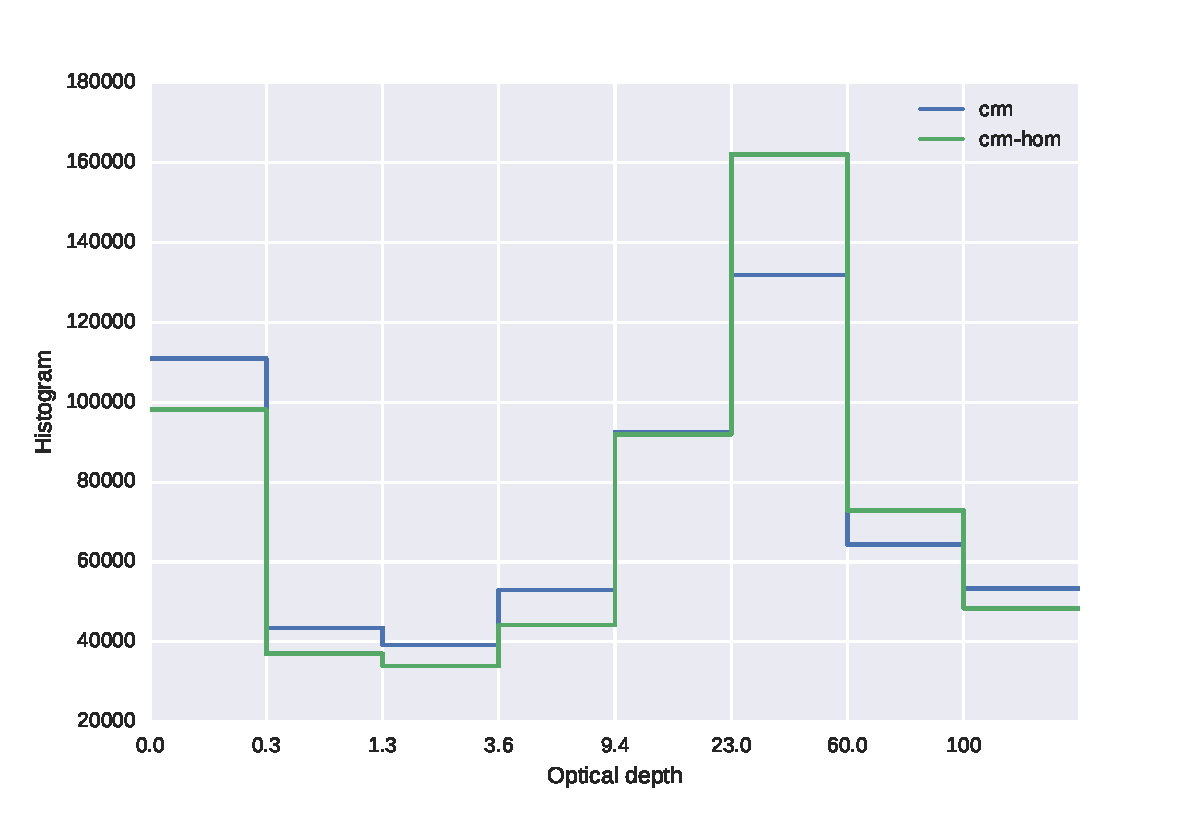
\includegraphics[width=\columnwidth]{graphics/taudist_hom.pdf}
\caption{Probability density function of cloud optical depth for a single day from the CRM and CRM-HOM cases.}
\label{sg_cldtau_distribution}
\end{figure}

The errors in total cloud area from the maximum-random overlap assumption alone are everywhere negative, showing that implementing maximum-random overlap tends to decrease the total vertically projected cloud area. The decrease in cloud area is a result of the maximum-random overlap assumption tending to overestimate the vertical correlation in adjacent cloudy layers, as discussed above and shown in Figure \ref{sg_overlap_mro}. This decrease is only -3\% cloud area in the global mean, but can reach values exceeding -10\% regionally, especially in the tropics. The decrease is largest for the low-topped cloud area, and high-topped cloud area actually increases slightly throughout some regions in middle to high latitudes. This is because the MISR simulator includes the tendency for MISR to ``see through'' optically thin upper cloud layers and retrieve cloud top heights of optically thicker lower cloud layers in cases involving multiple cloud layers. This is based on an optical depth threshold, where upper layers below a certain optical depth threshold are considered transparent, while layers above a certain threshold are opaque. Because increasing vertical correlation of cloudy layers tends to increase the cloud water path (and hence the cloud optical depth of those combined layers), the MRO assumption inflates the high-topped cloud area while decreasing the low-topped cloud area.

\begin{figure} 
\centering 
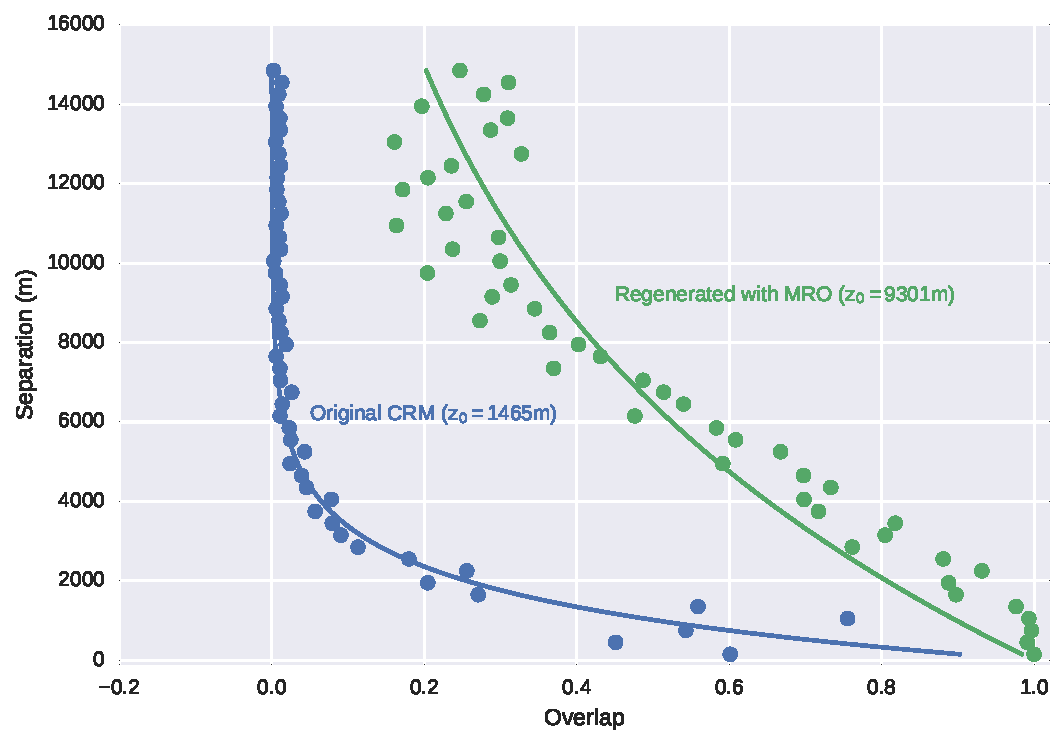
\includegraphics[width=\linewidth]{graphics/overlap_mro.pdf} 
\caption{Cloud occurrence overlap from original unmodified SP-CAM fields, and those with regenerated subcolumns assuming maximum-random overlap (MRO).} 
\label{sg_overlap_mro}
\end{figure}

The errors in MISR-simulated cloud area due separately to homogenizing cloud condensate and using MRO are mostly compensatory in the total cloud area, but combine to produce larger errors in high, middle, and low-topped cloud area. The effect on simulated high-topped clouds due to the two components of the error are both positive in sign, so that these components of the error combine to produce much larger errors in simulated high-topped cloud, with a 5\% cloud area increase in the global mean and an increase greater than 10\% cloud area throughout much of the deep tropics. The errors in high-topped cloud area are mostly compensated by a decrease in low-topped cloud, caused primarily by the errors due to using maximum-random overlap. The result is a decrease in simulated low-topped cloud of 4\% cloud area in the global average that, combined with the 2\% cloud area decrease in mid-topped clouds, nearly completely compensates the increase in high-topped cloud area. 

[TODO: comment on other simulators; show errors in joint/marginal histograms by region, especially for those regions identified as having large errors]
\begin{figure}
\centering
\caption{Cloud area errors from ISCCP}
\label{sg_cldisccp_errors}
\end{figure}

Figure \ref{sg_cldisccp_errors} shows errors in ISCCP-simulated cloud area by cloud type. These errors are qualitatively similar to the errors shown in Figure \ref{sg_cldmisr_maps_diff} for the MISR simulated cloud area by cloud type, with again an overestimation of total and high-topped cloud area due to homogenizing cloud condensate and an underestimation of total and low-topped cloud area due to using maximum-random overlap. [check this and elaborate]

\section{Sensitivity of simulated CloudSat diagnostics}

\begin{figure}
\centering
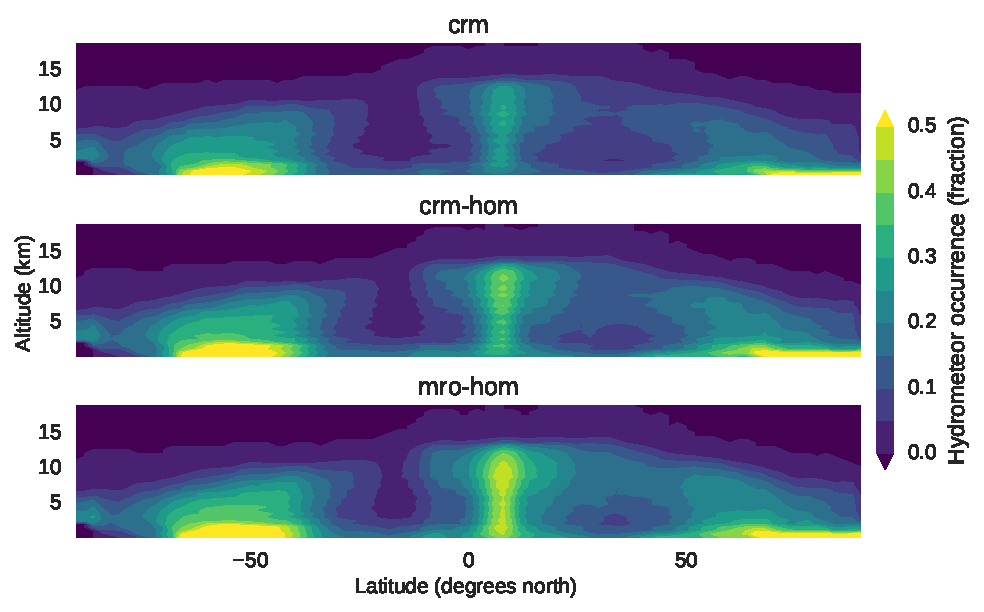
\includegraphics[width=\columnwidth]{graphics/hfba_mro-hom.pdf}
\caption{Hydrometeor occurence fraction by height}
\label{sg_hfba_zonal}
\end{figure}

\begin{figure}
\centering
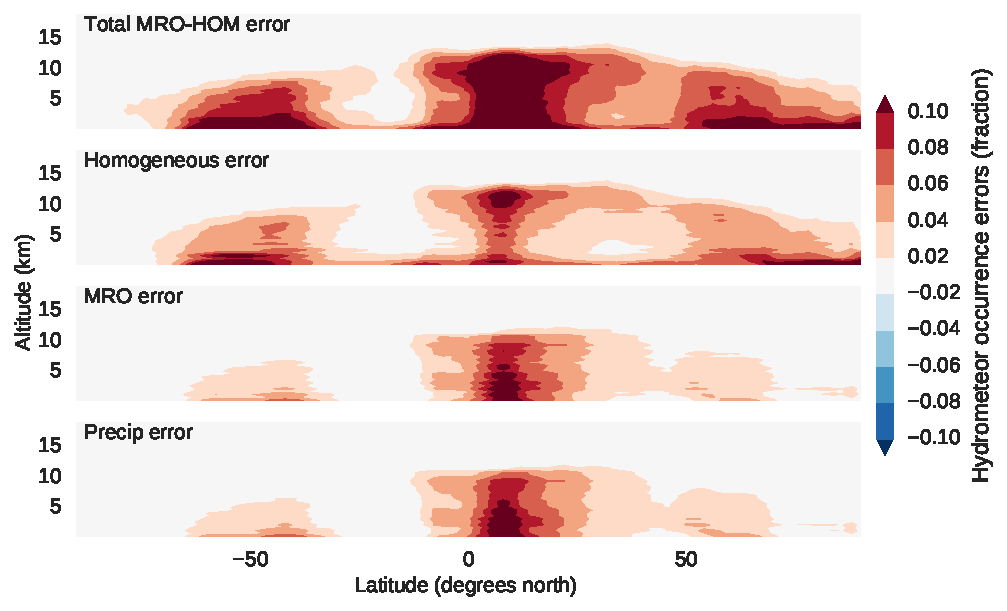
\includegraphics[width=\columnwidth]{graphics/hfba_mro-hom_errors.pdf}
\caption{Hydrometeor occurence fraction by height errors}
\label{sg_hfba_zonal_diff}
\end{figure}

The CloudSat simulator in COSP accounts for attenuation due to both hydrometeors and gases in the atmosphere. Because the CloudSat instrument has difficulty detecting hydrometeors with reflectivities below -27.5 dBZ, this threshold is often used when comparing simulated reflectivities from models to CloudSat observations \citep{marchand_et_al_2009}. The fraction of profiles with radar reflectivities above this threshold can be taken as a measure of the ``hydrometeor occurrence''. Figure \ref{sg_hfba_zonal} shows simulated zonal-mean hydrometeor occurrence profiles (the sum of occurrences of radar reflectivity bins with reflectivity  $Z_e > -27.5$ dBZ at a given height) from the CloudSat simulator outputs using the CRM, CRM-HOM, MRO-HOM, and MRO-HOM-PADJ fields, and Figure \ref{sg_hfba_zonal_diff} shows the errors in the MRO-HOM fields as well as the components of the errors due separately to homogenizing the condensate amounts and in using the maximum-random overlap assumption.  Homogenizing the cloud and precipitation condensate amounts and using the subcolumn generator in COSP both result in an increase in simulated hydrometeor occurrence at all altitudes. These errors are especially large in the deep tropics in the ITCZ and in both northern and southern hemisphere mid-latitudes. The errors due separately to homogenizing cloud and precipitation and to using the MRO scheme in COSP combine to produce larger total errors in hydrometeor occurrence than result from either component alone (top panel of Figure \ref{sg_hfba_zonal_diff}). 

These errors in hydrometeor occurrence are understand more fully by looking at the full reflectivity with height histograms. Figure \ref{sg_cfadDbze94_tropics} shows the simulated radar reflectivity with height histograms using the CRM, CRM-HOM, MRO-HOM, and MRO-HOM-PADJ cases for the northern hemisphere tropics (0 to 5 N latitude). While the histograms all show similar patterns of high frequency along a characteristic curve typical of reflectivity with height histograms \citep[e.g.,][]{marchand_et_al_2009}, the homogenized cases show substantially enhanced occurrence along the characteristic curve, and suppressed occurrence off of it where baseline occurrences are lower. This is more clear in Figure \ref{sg_cfadDbze94_tropics_diff}, which shows errors due to using homogeneous clouds and precipitation and to using SCOPS/PREC\_SCOPS to regenerate subcolumns. The source of these errors is again driven by the squeezing of the distribution of condensate that results from replacing the subgrid distribution of condensate with the gridbox averages, which effectively reduces the tails of the distribution by removing variability. This explains the apparent increase from low reflectivities to high reflectivities, but it would be expected that this would be accompanied by a corresponding decrease in the occurrence of very large reflectivities, which is \emph{not} seen in Figure \ref{sg_cfadDbze94_tropics_diff}. 

\begin{figure}
\centering
\caption{Reflectivity with height histograms for the NH Tropics [...].}
\label{sg_cfadDbze94_tropics}
\end{figure}

\begin{figure}
\centering
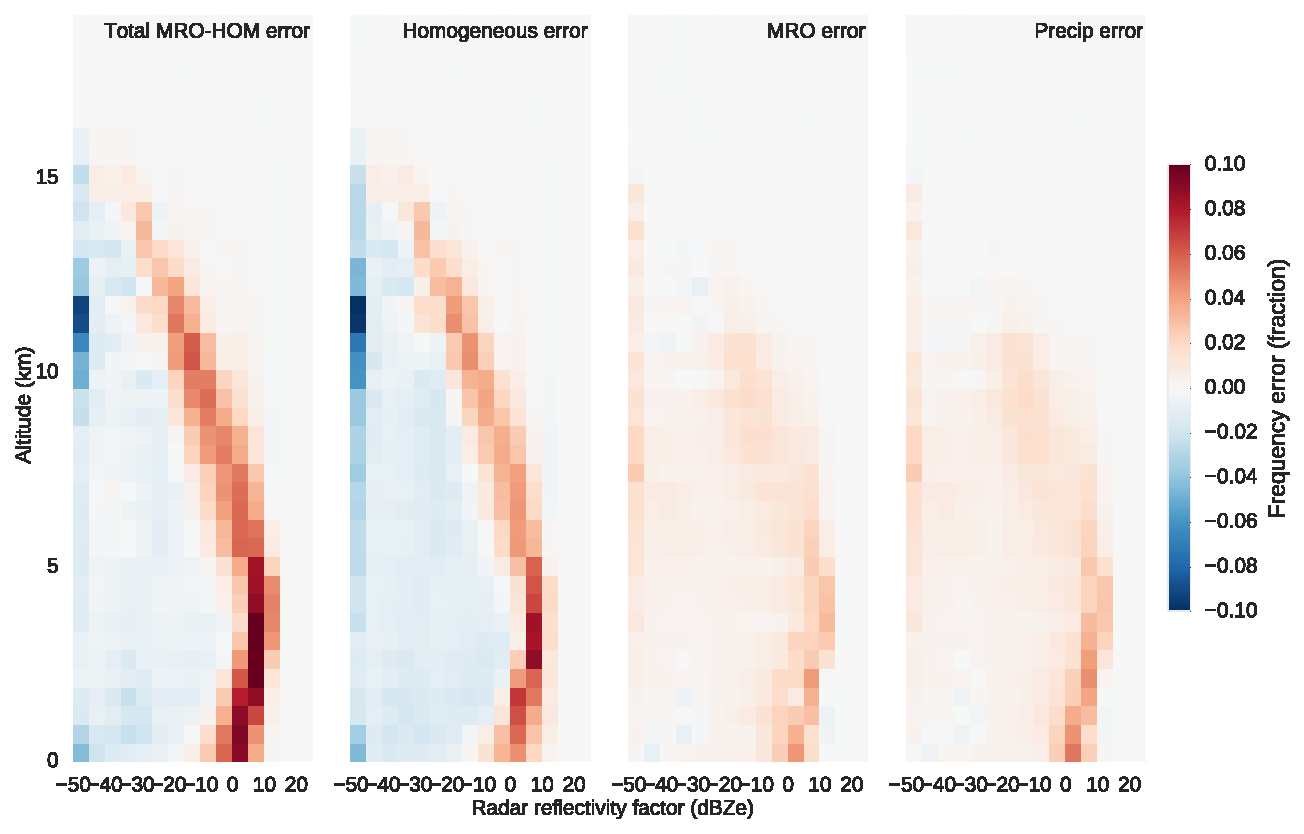
\includegraphics[width=\columnwidth]{graphics/cfadDbze94_mro-hom_errors.pdf}
\caption{Errors in reflectivity with height histograms for the NH Tropics [...].}
\label{sg_cfadDbze94_tropics_diff}
\end{figure}

This apparent inconsistency is explained by considering the attenuation of the radar signal by hydrometeors existing between each radar volume and the detector. The presence of such hydrometeors tends to decrease the radar signal, and in the presence of hydrometeors with large reflectivities this effect can be quite large. Because homogenizing the cloud and precipitation condensate decreases precisely those hydrometeors that would be expected to have such large reflectivities, homogenizing tends to simultaneously decrease the attenuation. Thus, while the total number of these highly reflective hydrometeors is decreased in the homogenized case, more of them would actually be visible to the radar due to decreased attenuation. The result is that the occurrence is increased along the characteristic curve, decreased for hydrometeors with lower reflectivity, but essentially unchanged for hydrometeors with large reflecitivity. This is demostrated for an example gridbox in Figure \ref{sg_cfadDbze94_testatt}, which shows the simulated reflectivity from both the CRM and CRM-HOM fields, but with attenuation turned on (top), and with attenuation turned off (bottom) for comparison. The histograms with attenuation turned off show precisely the squeezing of the distribution that we would have expected in the absence of attenuation.

\begin{figure}
\caption{Simulated reflectivity with height histograms for an example gridbox [...] using the CRM and CRM-HOM fields, with attenuation turned on (top) and with attenuation turned off (bottom).}
\label{sg_cfadDbze94_testatt}
\end{figure}

[much of this needs to be moved up and combined with the text above] These are all areas where the baseline hydrometeor occurrence is especially large (as seen in Figure \ref{sg_hfba_zonal}), and skewness in the distributions has a large impact on the volume of hydrometeors whose simulated reflectivity is greater than -27.5 dBZe. This effect is illustrated more clearly in Figure 11, which shows the errors in the reflectivity with height histograms for the northern hemisphere tropics (0 to 10 N). The figure shows the total errors in the MRO-HOM fields relative to the CRM fields, as well as the components of the error due to using homogeneous cloud properties (middle) and using the COSP subcolumn scheme to re-generate the subcolumns (right). The largest contribution to the error appears to be homogenizing the cloud properties, which results in a large increase in frequency along the characteristic curve where occurrence is maximized in the baseline CRM simulation and a decrease everywhere the occurrence is lower off of the characteristic curve in the baseline CRM simulation. The decrease in variability that occurs due to homogenization of the hydrometeor properties squeezes or narrows the distribution, increasing the total hydrometeor occurrence with , and increasing the hydrometeor occurrence diagnosed by the simulator.  Errors in CloudSat-simulated hydrometeor occurrence due to using the COSP subcolumn scheme to re-generate the subcolumns are less extensive than the errors due to homogenizing the hydrometeor properties, but can exceed 10\% frequency of occurrence in the tropics, and again lead to a false increase in the total hydrometeor occurrence. Figure 11 shows that the error is due to an increase in the occurrence of hydrometeors with all reflectivities, but especially due to an increase in the occurrence of columns with simulated radar reflectivity factor along the characteristic curve. The effect is more pronounced at low to mid-levels (altitude  km). This error is not surprising given the discussion in Section \ref{section_sg_framework} in the context of Figure 1, which shows that the COSP subcolumn generator can tend to overestimate the number of precipitating subcolumns. The fourth panel of Figure 9 shows the MRO component of the error when using the precipitation adjustment described in Section 2 (MRO-HOM-PADJ), and the MRO error is greatly reduced when we require the number of precipitating subcolumns to match the prescribed precipitation fraction. Likewise, the errors in simulated reflectivity with height due to the MRO alone are also small when we constrain the precipitation (not shown), leaving the homogeneous errors as dominating the total error in simulated CloudSat radar reflectivity. This suggests that the simulated CloudSat radar reflectivity is \emph{not} sensitive to the cloud overlap, but \emph{is} sensitive to the treatment of subgrid-scale precipitation.

[Discuss sensitivity to the threshold used? Line plots showing increases in profiles of occurrence for, e.g., NH Tropics?]

[need to quantify \emph{relative} errors, not just absolute errors?]

\section{Summary and discussion} Current global models do not resolve individual cloud elements, but rather represent the large-scale statistics by way of parameterization. But simulated satellite diagnostics (and radiative fluxes and heating rates) depend on the small-scale details of clouds. I have evaluated the sensitivity of simulated MISR and CloudSat satellite diagnostics from the CFMIP Observation Simulator Package to two assumptions: that cloud and precipitation properties are horizontally uniform on the scale of GCM gridboxes, and that individual cloud elements follow a maximum-random overlap. Because these assumptions are used to infer subgrid-scale cloud structure in model radiative transfer codes, these assumptions are also used by default in COSP to generate stochastic subcolumns on which the individual satellite instrument simulators are performed. However, others have shown that these assumptions lead to biases in calculated fluxes and heating rates, and it has been shown here that these assumptions also affect simulated MISR and CloudSat satellite diagnostics.  

The assumption of homogeneous cloud properties tends to inflate the simulated MISR cloud area (when counting all clouds with an optical depth greater than 0.3) because columns with small optical depths in the tail of the distribution are sometimes shifted to values above the cut-off threshold by the averaging. These errors occur primarily in high-topped clouds, and high-topped cloud occurrence can be overestimated by as much as 10\% cloud area in regions with a lot of high-topped optically thin cloud, such as in the tropical western pacific and other parts of the deep tropics. The global mean high-topped cloud error due to homogenizing the cloud properties is about 3\% cloud area, and the effect on total cloud area error is only 2\%.  The maximum-random overlap assumption tends to decrease the cloud cover because it overestimates the vertical alignment of vertically continuous clouds \citep{mace_and_benson-troth_2002, hogan_and_illingworth_2000, barker_2008}. This leads to a global mean underestimate in total cloud area of only 3\%, but with regional errors as large as 10\% cloud area, especially in the deep tropics.  The errors in cloud area due to homogeneous cloud properties and using the maximum-random overlap are generally opposite in sign, and result in a partial cancellation on the total error. The result is that the errors in total cloud area are less than 2\% in the global average, and regional errors in total cloud area are much smaller than for either of the two components of the error. However, errors in high and low-topped cloud area due to the two components are additive, such that the total errors in high and low-topped clouds are larger than they are for either the homogeneous or MRO components. High-topped cloud is overestimated by 5\% cloud area, and low-topped cloud is underestimated by 4\% cloud area in the global mean. Regional errors are even larger, and high-topped cloud errors reach 10\% cloud area or more, especially in the tropical western pacific, the Indian Ocean, and throughout the tropics.

The sensitivity in MISR-simulated total cloud area identified here is generally less than errors in cloud area identified in current GCMs \citep{kay_et_al_2012, klein_et_al_2013, bodas-salcedo_et_al_2011}, and on the order of the spread in estimates of total cloud area from satellite remote sensing retrievals \cite{marchand_et_al_2010, pincus_et_al_2012}. However, the regional errors in MISR-simulated cloud area by cloud top height identified here are large, and exceed the uncertainty in MISR-retrieved high-topped cloud area, which is estimated to be on the order of 5\% cloud area regionally, as shown in Chapter \ref{me_chapter} and \cite{hillman_et_al_2016}. Thus, the sensitivity of MISR-simulated cloud area to homogeneous cloud condensate and maximum-random overlap cannot be ignored, especially as representations of clouds in GCMs improve. 

[comment also on distribution of optical depth?]

Errors in simulated CloudSat radar reflectivity are found to be sensitive to the treatment of subcolumn cloud and precipitation condensate, but much less sensitive to the treatment of cloud overlap. Homogenizing the cloud and precipitation condensate leads to a narrowing of the distribution of simulated radar reflectivity, making the more frequently occurring reflectivities in the baseline simulation even more frequently occurring in the homogenized simulation. This tends to decrease the occurrence of columns with small radar reflectivity, while increasing the occurrence of columns with large radar reflectivity. Similar to the MISR simulator, employing a reflectivity cut-off to determine hydrometeor occurrence (for the purpose of making consistent comparisons with CloudSat) then results in an apparent increase in the hydrometeor occurrence when homogenizing the cloud and precipitation properties, and an apparent increase in precipitation occurrence. The increase in simulated hydrometeor occurrence fraction reaches a value of 10\% in high altitudes in the tropics and in low altitudes in mid to high-latitudes.  

Using the subcolumn generator currently implemented in COSP (as of version 1.4) leads to further errors in simulated CloudSat radar reflectivity and hydrometeor occurrence that combine with the errors due to homogenizing the cloud and precipitation condensate to produce even larger total errors that reach 10\% frequency of occurrence at all altitudes throughout the tropics. Much of this error is due to the fact that precipitation has a relatively large reflectivity compared with clouds, and the subcolumn precipitation scheme implemented in COSP tends to overestimate the number of precipitating subcolumns. Using this subcolumn scheme then tends to increase the number of columns with large radar reflectivity, and thus increases the simulated hydrometeor occurrence.  Constraining the number of precipitating subcolumns by the precipitation fraction greatly reduces errors in simulated hydrometeor occurrence. The ability to constrain the subcolumn precipitation by the precipitation fraction will be included in future versions of COSP (Y. Zhang, personal communication), and will be explored further in the following chapter [???]. The remaining errors due to maximum-random cloud overlap alone are small, with hydrometeor occurrence errors everywhere less than 4\% in the zonal mean.

The errors in simulated CloudSat radar reflectivity factor and hydrometeor occurrence due to the homogenous cloud and precipitation assumptions are troubling, and show that subgrid-scale cloud and precipitation variability needs to be better represented in COSP in order to create more consistent comparisons between model-diagnosed and satellite-retrieved cloud statistics. The following chapter explores the possibility of reducing these errors with an improved subcolumn generator framework, which includes both a more realistic treatment of overlap and heterogeneous condensate.

%% END OF CHAPTER
